% =====================================================================
% BLADE poster -- Penn State theme (PSUPoster), solid Beaver Blue, DIN A0 portrait.
% Build: latexmk blade-poster.tex   (XeLaTeX + biber, see .latexmkrc)
% Using this as a template: see README.md.
%
% This file holds the poster settings, title block and content. Look and feel live in:
%   beamerthemePSUPoster.sty   header, footer, outer blocks (psublock, psufinalblock, plainblock)
%   beamercolorthemepsu.sty    color palette (psu-beaver, psu-pugh, psu-pink, ...)
%   preamble/packages.tex      packages and fonts
%   preamble/bibliography.tex  compact reference-list style
%   preamble/macros.tex        paper notation (\method, \Loss, ...)
%   preamble/boxes.tex         inner boxes (probcard, compblock, benchtile, \chip, \bignum, ...)
%
% Content rows below (search for "Row N"):
%   Row 1 motivation | Row 2 method | Row 3 setup + key result
%   Row 3 experiments | Row 6 references  (old Rows 3-5 parked in parked/)
% =====================================================================
\documentclass[final,svgnames,english]{beamer}
\usepackage[english]{babel}

\usepackage[orientation=portrait,size=a0,scale=1.125]{beamerposter}
\usetheme{PSUPoster}

% =====================================================================
% Packages and fonts. Needs XeLaTeX (fontspec/mathspec).
% =====================================================================
\usepackage{amsmath,amsthm, amssymb, latexsym}
\usepackage{mathspec}
% Penn State brand typefaces: Roboto (body) and Roboto Slab (headings), both ship with TeX Live.
\defaultfontfeatures{Ligatures=TeX}
\setmainfont{Roboto}[Extension=.ttf, UprightFont=*-Regular, BoldFont=*-Bold,
  ItalicFont=*-Italic, BoldItalicFont=*-BoldItalic]
\setsansfont{Roboto}[Extension=.ttf, UprightFont=*-Regular, BoldFont=*-Bold,
  ItalicFont=*-Italic, BoldItalicFont=*-BoldItalic]
\setfontfamily\headingfont{RobotoSlab}[Extension=.otf, UprightFont=*-Regular, BoldFont=*-Bold]
\IfFontExistsTF{Fira Code}
  {\setmonofont{Fira Code}[Scale=0.74]}
  {\setmonofont{FiraMono}[Extension=.otf, UprightFont=*-Regular, BoldFont=*-Bold, Scale=0.74]}
\setmathrm[Extension=.ttf, UprightFont=*-Regular, BoldFont=*-Bold,
  ItalicFont=*-Italic, BoldItalicFont=*-BoldItalic]{Roboto}

\usepackage{graphicx}
\usepackage{booktabs}
\usepackage{colortbl}
\usepackage{qrcode}
\usepackage{adjustbox}
\usepackage{xspace}
\usepackage{nicefrac}
\usepackage{multiobjective}
% fontawesome7 needs TeX Live 2025+; fall back to fontawesome5 on older systems.
\IfFileExists{fontawesome7.sty}{\usepackage{fontawesome7}}{\usepackage{fontawesome5}}
\urlstyle{tt}
\usepackage{setspace}
\usepackage{multicol}

\usepackage{tikz}
\usetikzlibrary{calc, backgrounds, arrows, arrows.meta, shapes, positioning, fit}

% =====================================================================
% Bibliography: compact numeric style (first author, title, year).
% Bib file: references.bib. The list is printed in the last row of the poster.
% =====================================================================
\usepackage[backend=biber, bibstyle=numeric, autocite=superscript, defernumbers=true, citestyle=numeric,
  maxbibnames=1, minbibnames=1, giveninits=true]{biblatex}
\usepackage{csquotes}

\makeatletter
\RequireBibliographyStyle{numeric}
\DeclareFieldFormat{labelnumberwidth}{#1.}
\makeatother

% Print titles exactly as in the paper's bib (biblatex-apa would sentence-case them).
\DeclareFieldFormat{apacase}{#1}
\DeclareFieldFormat{url}{url\addcolon\space\url{#1}}

\renewbibmacro*{url+urldate}{%
  \ifthenelse{\iffieldundef{url}\OR\NOT\iffieldundef{doi}}
  {}
  {\iffieldundef{urlyear}
    {}
    {\setunit{\addspace}}%
\iffieldundef{url}{}{\printfield{url}\renewcommand*{\finentrypunct}{\relax}}}}

\addbibresource{references.bib}
% Poster references: first author et al., title, year.
\AtEveryBibitem{\clearfield{url}\clearfield{doi}\clearfield{pages}\clearfield{volume}
  \clearfield{number}\clearlist{publisher}\clearlist{location}\clearname{editor}\clearfield{eventtitle}
  \clearfield{booktitle}\clearfield{journaltitle}\clearfield{month}\clearlist{organization}\clearlist{institution}}
\AtEveryBibitem{\clearfield{isbn}\clearfield{issn}}
\renewbibmacro{in:}{}
% Narrow label column for the compact poster bibliography.
\defbibenvironment{bibliography}
  {\list{\printfield[labelnumberwidth]{labelnumber}}
    {\setlength{\leftmargin}{1.5em}\setlength{\labelwidth}{1.3em}\setlength{\labelsep}{0.2em}
     \setlength{\itemsep}{\bibitemsep}\setlength{\parsep}{0pt}}
   \renewcommand*{\makelabel}[1]{##1\hss}}
  {\endlist}
  {\item}

\AtBeginBibliography{\setstretch{1.1}\raggedright}
% No stretchable glue inside URLs (otherwise they print as "https : / / ...").
\setlength{\biburlbigskip}{0mu}
\setlength{\biburlnumskip}{0mu}
\setlength{\biburlucskip}{0mu}
\setlength{\biburllcskip}{0mu}

% =====================================================================
% Paper-specific macros. Replace these with your own paper's notation.
% =====================================================================
\newcommand{\method}{\textbf{BLADE}\xspace}
\newcommand{\Loss}{\mathcal{L}}
\newcommand{\Dforget}{\mathcal{D}_\text{forget}}
\newcommand{\Dretain}{\mathcal{D}_\text{retain}}
\newcommand{\best}[1]{\textbf{\textcolor{psu-pink}{#1}}}
\newcommand{\up}{$\uparrow$}
\newcommand{\down}{$\downarrow$}

% =====================================================================
% Content boxes used inside the poster blocks (all tcolorbox, PSU colors).
% The outer blocks (psublock, psufinalblock, plainblock, tldrbox) live in
% beamerthemePSUPoster.sty; these are the smaller pieces placed inside them.
% =====================================================================

% ---------------------------------------------------------------------
% Highlight boxes
% ---------------------------------------------------------------------
\newtcolorbox{callout}{%
  enhanced, sharp corners, colback=psu-beaver-tint, width=\linewidth,
  colframe=psu-navy, boxrule=0pt, leftrule=7.4pt,
  left=11pt, right=5pt, top=9pt, bottom=9pt,
before skip=11pt, after skip=5pt}

\newtcolorbox{takeaway}{%
  enhanced, sharp corners, colback=psu-pugh-tint, width=\linewidth,
  colframe=psu-beaver, boxrule=0pt, leftrule=7.4pt,
  left=11pt, right=5pt, top=9pt, bottom=9pt,
before skip=11pt, after skip=5pt}

\newtcolorbox{inform}{%
  enhanced, sharp corners, colback=psu-beaver-tint, width=\linewidth,
  colframe=psu-beaver, boxrule=0pt, leftrule=7.4pt,
  left=11pt, right=5pt, top=9pt, bottom=9pt,
before skip=11pt, after skip=5pt}

% block for the main findings of the paper
% Header band: one solid Pugh Blue band for every finding (no gradient).
\newtcolorbox{findingblock}[2]{%
  enhanced, sharp corners, colback=psu-#2!3, width=\linewidth,
  colframe=psu-#2, boxrule=0.47pt, leftrule=7.4pt, titlerule=0pt, title={#1},
  colbacktitle=psu-pugh!70, coltitle=psu-navy, fonttitle=\bfseries,
  lefttitle=11pt, toptitle=5pt, bottomtitle=5pt,
  left=11pt, right=5pt, top=6pt, bottom=9pt,
before skip=5pt, after skip=5pt}

% Numbered circle, e.g. \circnum{1} to tag a method component.
% Reset node options: inside a TikZ node the nested picture inherits its size and frame.
\newcommand{\circnum}[1]{\tikz[baseline=(n.base)]\node[circle, fill=psu-pugh, draw=none,
  text width={}, minimum width=0pt, minimum height=0pt, line width=0pt, align=center,
  text=psu-navy, inner sep=0.12em, font=\bfseries\footnotesize] (n) {#1};}

% Failure-mode card (motivation) and component box (method); see figs/tikz-problems.tex.
\newtcolorbox{probcard}[1]{%
  enhanced, sharp corners, colback=psu-pink!4, colframe=psu-pink, boxrule=2pt,
  colbacktitle=psu-pink, coltitle=psu-white, fonttitle=\bfseries, title={#1},
  equal height group=prob,
  left=6pt, right=6pt, top=10pt, bottom=8pt, toptitle=6pt, bottomtitle=6pt,
  before skip=6pt, after skip=6pt}
% Optional argument: extra tcolorbox keys, e.g. a different equal height group.
\newtcolorbox{compblock}[2][]{%
  enhanced, sharp corners, colback=psu-white, width=\linewidth,
  colframe=psu-beaver, boxrule=0.47pt, leftrule=7.4pt, titlerule=0pt,
  title={\strut #2}, equal height group=comp,
  colbacktitle=psu-pugh!70, coltitle=psu-navy, fonttitle=\bfseries\psuhighsize,
  lefttitle=11pt, righttitle=11pt, toptitle=8pt, bottomtitle=8pt,
  left=14pt, right=10pt, top=10pt, bottom=12pt,
  before skip=12pt, after skip=6pt, #1}
\newcommand{\fixtag}[1]{\tcbox[on line, enhanced, frame hidden, colback=psu-pink, coltext=psu-white,
  arc=12pt, left=8pt, right=8pt, top=3pt, bottom=3pt, fontupper=\small\bfseries]{fixes #1}}

% Benchmark tile (experiments), baseline chip, and headline number (key result).
\newtcolorbox{benchtile}[1]{%
  enhanced, sharp corners, colback=psu-beaver-tint, colframe=psu-beaver, boxrule=2pt,
  colbacktitle=psu-beaver, coltitle=psu-white, fonttitle=\bfseries, title={#1},
  halign=center, halign title=center, equal height group=bench,
  left=6pt, right=6pt, top=8pt, bottom=8pt, toptitle=6pt, bottomtitle=6pt,
  before skip=6pt, after skip=6pt}
\newcommand{\chip}[1]{\tcbox[on line, enhanced, frame hidden, colback=psu-pugh-tint, coltext=psu-navy,
  arc=10pt, left=7pt, right=7pt, top=3pt, bottom=3pt, fontupper=\bfseries]{#1}}
\newcommand{\bignum}[3]{%
  {\color{#1}\LARGE\bfseries #2}\\[0.1ex]{\small #3}\par\vspace{1.6ex}}


% ---------------------------------------------------------------------
% Title block (rendered in the header by beamerthemePSUPoster.sty)
% ---------------------------------------------------------------------
\title{BLADE: Bilevel Low-rank Augmented-Lagrangian Erasure for LLM Unlearning}
\author{Md Toufikuzzaman\textsuperscript{1}, Ahmad Mousavi\textsuperscript{2}, and Dongwon Lee\textsuperscript{1}}
\institute[]{\textsuperscript{1}The Pennsylvania State University, USA \quad \textsuperscript{2}American University, USA\\[0.2ex]
  \{mpt5763, dongwon\}@psu.edu, \ mousavi@american.edu}

\begin{document}
\begin{frame}[t,fragile]{}
  \vspace{0.3em}
  \begin{columns}[T]
    % Forcing left margin
    \begin{column}{0.01\linewidth}
    \end{column}

    % Content: full-width rows, read left to right
    \begin{column}{0.98\linewidth}

      % ======================= Row 1: motivation =======================
      \begin{columns}[T,onlytextwidth]
        \begin{column}{0.52\linewidth}
          \begin{psublock}[equal height group=r1]{Problem Overview}
            \centering
            \adjustbox{width=0.82\linewidth}{% What unlearning is (paper, Problem Setup): from a deployed model, make outputs on D_forget
% high-entropy while keeping the retain cross-entropy below a budget epsilon. No retraining.
\begin{tikzpicture}[
    model/.style={draw=psu-beaver, fill=psu-beaver, text=white, rounded corners=12pt,
      minimum width=6cm, minimum height=3.8cm, align=center, font=\bfseries},
    data/.style={rounded corners=10pt, minimum height=1.8cm, inner xsep=12pt, align=center,
      text=white, font=\small\bfseries},
    flow/.style={-{Triangle[length=18pt,width=20pt]}, line width=4pt, color=psu-beaver},
  ]
  \node[model] (m0) at (0,0) {\Large\faRobot\\[0.4ex]LLM $M_{\theta_0}$};
  \node[draw=psu-navy, line width=3pt, fill=psu-pugh-tint, text=psu-navy, rounded corners=22pt,
    minimum height=2.4cm, inner xsep=18pt, font=\bfseries] (u) at (9.6,0) {unlearning};
  \node[model] (m1) at (19.2,0) {\Large\faRobot\\[0.4ex]unlearned $M_{\theta}$};
  \draw[flow] (m0) -- (u);
  \draw[flow] (u) -- (m1);
  \node[data, fill=psu-pink] (df) at (5.0,3.9) {\faFile*\ \ $\mathcal{D}_\text{forget}$: remove};
  \node[data, fill=psu-beaver] (dr) at (14.4,3.9) {\faFile*\ \ $\mathcal{D}_\text{retain}$: keep};
  \draw[-{Stealth[length=14pt]}, line width=3pt, psu-pink] (df.south) -- (u.north west);
  \draw[-{Stealth[length=14pt]}, line width=3pt, psu-beaver] (dr.south) -- (u.north east);
  \node[anchor=west, align=left, font=\small] at ([xshift=0.6cm, yshift=0.8cm]m1.east)
    {\textcolor{psu-pink}{\faTimes}\ \ $\mathcal{D}_\text{forget}$};
  \node[anchor=west, align=left, font=\small] at ([xshift=0.6cm, yshift=-0.8cm]m1.east)
    {\textcolor{psu-beaver}{\faCheck}\ \ $\mathcal{D}_\text{retain}$};
\end{tikzpicture}
}
            \vspace{2ex}

            \adjustbox{width=0.9\linewidth}{% Unlearning requests keep arriving after deployment.
\begin{tikzpicture}[
    req/.style={circle, fill=psu-pink, text=white, minimum size=2.3cm, inner sep=0pt, font=\Large},
    lbl/.style={below=0.25cm, text=psu-navy, font=\footnotesize},
  ]
  \node[draw=psu-beaver, fill=psu-beaver, text=white, rounded corners=10pt, minimum height=2.3cm,
    inner sep=14pt, font=\bfseries] (llm) at (0,0) {\faRobot\ \ deployed LLM};
  \draw[-{Triangle[length=18pt,width=20pt]}, line width=4pt, psu-beaver]
    (llm.east) -- ++(0.64\linewidth,0) node[right, text=psu-navy, font=\small] {time};
  \foreach \x/\ic/\t in {0.05/\faIcon{user-shield}/privacy (GDPR),
                          0.215/\faCopyright/copyright,
                          0.38/\faBiohazard/hazardous,
                          0.545/\faNewspaper/misinformation} {
    \node[req] (r) at ([xshift=\x\linewidth+1.3cm]llm.east) {\ic};
    \node[lbl] at (r.south) {\t};
  }
\end{tikzpicture}
}
          \end{psublock}
        \end{column}
        \begin{column}{0.46\linewidth}
          \begin{psublock}[equal height group=r1]{Objectives}
            {\psuhighsize\bfseries\color{psu-navy}Designing an unlearning method that is \dots}\\[1.2ex]
            \setlength{\tabcolsep}{6pt}\renewcommand{\arraystretch}{1.6}
            \begin{tabular*}{\linewidth}{@{}c@{\extracolsep{\fill}}ll@{}}
              {\Large\color{psu-beaver}\faBalanceScale} & {\psuhighsize\color{psu-beaver}\textbf{Balanced}} & Forgets with minimal model degradation \\
              {\Large\color{psu-beaver}\faIcon{expand-arrows-alt}} & {\psuhighsize\color{psu-beaver}\textbf{Scalable}} & Stays stable as forget set grows \\
              {\Large\color{psu-beaver}\faIcon{sync-alt}} & {\psuhighsize\color{psu-beaver}\textbf{Sustainable}} & Handles repeated unlearning requests \\
              {\Large\color{psu-beaver}\faShield*} & {\psuhighsize\color{psu-beaver}\textbf{Robust}} & Resists extraction, jailbreak and membership attacks \\
              {\Large\color{psu-beaver}\faMicrochip} & {\psuhighsize\color{psu-beaver}\textbf{Efficient}} & Inexpensive finetuning with smaller memory footprint \\
            \end{tabular*}
          \end{psublock}
        \end{column}
      \end{columns}

      % ======================= Row 2: method =======================
      \begin{psublock}{BLADE: Method}
        \begin{columns}[T]
          \begin{column}{0.42\linewidth}
            \begin{compblock}[equal height group=r2top, valign=center]{Formulation}
              \centering
              \adjustbox{width=0.8\linewidth}{$\begin{array}{c}
                \displaystyle
                \underbrace{\min_{\theta}\ \Loss_{\text{fgt}}(\theta^*;\Dforget)}_{\textcolor{psu-pink}{\textbf{Forget}}}
                \quad\text{s.t.}\quad
                \underbrace{\Loss_{\text{CE}}(\theta^*;\Dretain) \le \varepsilon}_{\textcolor{psu-navy}{\textbf{Retain budget}}}
                \\[6ex]
                \displaystyle
                \underbrace{\theta^* \approx \argmin_{\theta}\ \Loss_{\text{CE}}(\theta;\Dretain)}_{\textcolor{psu-beaver}{\textbf{Repair (inner)}}}
                \qquad
                \underbrace{W' = W_0 + \tfrac{\alpha}{r}BA}_{\textcolor{psu-beaver}{\textbf{LoRA},\ W_0\ \text{frozen}}}
              \end{array}$}
            \end{compblock}
          \end{column}
          \begin{column}{0.56\linewidth}
            \begin{compblock}[equal height group=r2top]{One training step}
              \centering
              \adjustbox{max width=\linewidth}{% One BLADE outer step: inner retain repair -> constrained forget step -> asymmetric dual update.
\begin{tikzpicture}[
    font=\small,
    stage/.style={draw=#1, fill=#1!8, line width=2.5pt, rounded corners=10pt,
      text width=0.27\linewidth, minimum height=5.6cm, align=center, inner sep=12pt},
    flow/.style={-{Triangle[length=16pt,width=18pt]}, line width=3.5pt, color=psu-beaver},
  ]
  \node[stage=psu-beaver] (inner) {%
    {\color{psu-beaver}\textbf{\circnum{1} Inner loop $\times K$}}\\[0.3ex]
    \textbf{Retain repair}, fast $\eta_{\text{in}}$\\[0.5ex]
    $\theta \leftarrow \theta - \eta_{\text{in}}\nabla_\theta \mathcal{L}_{\text{CE}}(\mathcal{B}_{\text{ret}})$};
  \node[stage=psu-navy, right=0.045\linewidth of inner] (outer) {%
    {\color{psu-navy}\textbf{\circnum{2} Outer step}}\\[0.3ex]
    \textbf{Constrained forgetting}, slow $\eta_{\text{out}}$\\[0.5ex]
    $\mathcal{L}_{\text{fgt}} + \lambda r + \tfrac{\rho}{2}[r]_+^2$};
  \node[stage=psu-pink, right=0.045\linewidth of outer] (dual) {%
    {\color{psu-pink}\textbf{\circnum{3} Dual ratchet}}\\[0.3ex]
    \textbf{Adapt} $\lambda$ to violations\\[0.5ex]
    $r{>}0:\ \lambda \mathrel{+}= \rho|r|$\\
    $r{\le}0:\ \lambda \mathrel{-}= \alpha\rho|r|$};
  \draw[flow] (inner) -- (outer);
  \draw[flow] (outer) -- (dual);
  \draw[flow] (dual.south) -- ++(0,-1.6cm) -| node[pos=0.25, fill=white, inner sep=6pt]
    {next step $t{+}1$, \ $r = \mathcal{L}_{\text{CE}}(\mathcal{B}'_{\text{ret}}) - \varepsilon$ on a fresh batch} (inner.south);
  \begin{scope}[on background layer]
    \node[draw=psu-beaver!60, dashed, line width=2pt, rounded corners=14pt,
      fit=(inner)(outer)(dual), inner xsep=18pt, inner ysep=2.9cm, yshift=-0.85cm,
      label={[anchor=north east, inner sep=12pt, text=psu-beaver, font=\footnotesize]north east:%
        \textbf{LoRA adapters only} --- $W_0$ frozen, ${\sim}0.2\%$ of 7B params trainable}] {};
  \end{scope}
\end{tikzpicture}
}
            \end{compblock}
          \end{column}
        \end{columns}

        \begin{columns}[T]
          \begin{column}{0.325\linewidth}
            \begin{compblock}{Repair-first principle}
              \centering
              \adjustbox{max width=\linewidth}{% Repair-first (qualitative): each small forget step raises retain loss,
% the following K fast repair steps bring it back before the next forget step.
% Drawn at print size (about 24 cm wide) so labels print at their nominal size.
\begin{tikzpicture}[x=0.8cm, y=0.8cm, font=\normalsize]
  \def\lo{1.0} \def\hi{3.4} \def\eps{5.0}
  \draw[-{Stealth[length=14pt]}, line width=2.5pt, psu-navy] (0,0) -- (20.6,0) node[right] {steps};
  \draw[-{Stealth[length=14pt]}, line width=2.5pt, psu-navy] (0,0) -- (0,6.4) node[above right] {retain loss};
  \draw[dashed, line width=3pt, psu-navy] (0,\eps) -- (20,\eps) node[above left] {budget $\varepsilon$};
  \foreach \c in {0,1,2} {
    \pgfmathsetmacro{\s}{0.6+6.4*\c}
    \draw[line width=6pt, psu-pink] (\s,\lo) -- (\s+0.8,\hi);
    \draw[line width=6pt, psu-beaver]
      (\s+0.8,\hi) -- (\s+2.0,\hi) -- (\s+2.0,{\hi-0.6}) -- (\s+3.2,{\hi-0.6})
      -- (\s+3.2,{\hi-1.2}) -- (\s+4.4,{\hi-1.2}) -- (\s+4.4,{\hi-1.8})
      -- (\s+5.6,{\hi-1.8}) -- (\s+5.6,\lo) -- (\s+6.4,\lo);
  }
  \node[anchor=north, font=\bfseries] at (10,-0.4)
    {\textcolor{psu-pink}{\rule[0.25ex]{1.4cm}{6pt}\ forget step}\qquad
     \textcolor{psu-beaver}{\rule[0.25ex]{1.4cm}{6pt}\ repair $\times K$}};
\end{tikzpicture}
}\\[0.4ex]
              $\displaystyle \theta \leftarrow \theta - \eta_{\text{in}}\nabla_\theta\Loss_{\text{CE}}(\mathcal{B}_{\text{ret}})
                \ \times K$\par\vspace{0.4ex}
              \raggedright
              \begin{itemize}
                \item Forget and retain are \textbf{entangled}
                \item Forget is \textbf{destructive} by nature
                \item \textbf{Anchor} forget by retain
              \end{itemize}
            \end{compblock}
          \end{column}
          \begin{column}{0.325\linewidth}
            \begin{compblock}{Asymmetric ALM}
              \centering
              \adjustbox{max width=\linewidth}{% Asymmetric dual update (qualitative). A symmetric update lets lambda fall as fast as it rose,
% so retain violations recur and lambda oscillates; BLADE decays alpha times slower and stays up.
% Drawn at print size (about 24 cm wide) so labels print at their nominal size.
\begin{tikzpicture}[x=0.8cm, y=0.8cm, font=\normalsize]
  \def\lo{0.8} \def\hi{4.0}
  \draw[-{Stealth[length=14pt]}, line width=2.5pt, psu-navy] (0,0) -- (20.6,0) node[right] {steps};
  \draw[-{Stealth[length=14pt]}, line width=2.5pt, psu-navy] (0,0) -- (0,6.6) node[above] {$\lambda$};
  % symmetric: same slope up and down, back to the start, violated again
  \draw[line width=4pt, psu-black!40, dashed]
    (0.2,\lo) -- (3,\lo) -- (4,\hi) -- (5,\lo) -- (8,\lo) -- (9,\hi) -- (10,\lo)
    -- (13,\lo) -- (14,\hi) -- (15,\lo) -- (20,\lo);
  % BLADE: same rise, then a slow decay
  \draw[line width=6pt, psu-beaver] (0.2,\lo) -- (3,\lo) -- (4,\hi) -- (20,3.3);
  \fill[psu-pink] (3,0) ++(-0.4,-0.75) -- ++(0.8,0) -- ++(-0.4,0.7) -- cycle;
  \node[text=psu-pink, font=\bfseries, anchor=north west] at (3.6,-0.15) {$r>0$: violation};
  % legend
  \draw[line width=6pt, psu-beaver] (1.2,5.8) -- (2.8,5.8);
  \node[text=psu-beaver, font=\bfseries, anchor=west] at (3.0,5.8) {\method};
  \draw[line width=4pt, psu-black!40, dashed] (9.6,5.8) -- (11.2,5.8);
  \node[text=psu-black!60, font=\bfseries, anchor=west] at (11.4,5.8) {symmetric};
\end{tikzpicture}
}\\[0.4ex]
              $\displaystyle \Loss_{\text{outer}} = \Loss_{\text{fgt}} + \lambda r + \tfrac{\rho}{2}[r]_+^2,
                \quad r = \Loss_{\text{ret}} - \varepsilon$\par\vspace{0.4ex}
              \raggedright
              \begin{itemize}
                \item \textbf{Constrained} forget under retain
                \item $\lambda$ grows fast, decays slowly
              \end{itemize}
            \end{compblock}
          \end{column}
          \begin{column}{0.325\linewidth}
            \begin{compblock}{Clamped entropy}
              \centering
              \adjustbox{max width=\linewidth}{% Per-token forget loss as a function of the token's output entropy H(p_t).
% Clamped: max(0, tau*Hmax - H) with a zero-gradient deadzone; unclamped (tau = 1) keeps pushing.
% Drawn at print size (about 24 cm wide) so labels print at their nominal size.
\begin{tikzpicture}[x=0.8cm, y=0.8cm, font=\normalsize]
  \def\W{17}    % x extent = H_max
  \def\T{11}    % tau * H_max
  \def\Hgt{6}
  \fill[psu-pugh-tint] (\T,0) rectangle (\W,\Hgt);
  \node[text=psu-beaver, font=\bfseries] at ({(\T+\W)/2},{0.7*\Hgt}) {deadzone};
  \draw[-{Stealth[length=14pt]}, line width=2.5pt, psu-navy] (0,0) -- (\W+0.8,0)
    node[right] {$H(p_t)$};
  \draw[-{Stealth[length=14pt]}, line width=2.5pt, psu-navy] (0,0) -- (0,\Hgt+1.6)
    node[above] {loss};
  \draw[dashed, line width=3.5pt, psu-black!40] (0,{0.95*\Hgt}) -- (\W,0);
  \node[anchor=south west, font=\bfseries] at (1.4,\Hgt+0.15)
    {\textcolor{psu-black!60}{unclamped:} \textcolor{psu-pink}{over-forgetting}};
  \draw[line width=6pt, psu-pink] (0,{0.95*\Hgt*\T/\W}) -- (\T,0) -- (\W,0);
  \node[text=psu-pink, anchor=south west, font=\bfseries] at (\T+0.2,0.25) {clamped};
  \draw[line width=2pt] (\T,0.3) -- (\T,-0.3) node[below] {$\tau\log V$};
  \draw[line width=2pt] (\W,0.3) -- (\W,-0.3) node[below] {$\log V$};
\end{tikzpicture}
}\\[0.4ex]
              $\displaystyle \Loss_{\text{fgt}} = \tfrac{1}{N}\textstyle\sum_{t} \max\!\big(0,\, \tau\log V - H(p_t)\big)$\par\vspace{0.4ex}
              \raggedright
              \begin{itemize}
                \item $\nabla = 0$ \textbf{once forgotten}
                \item \textbf{Bounded} and reference-free
              \end{itemize}
            \end{compblock}
          \end{column}
        \end{columns}
      \end{psublock}

      % ======================= Row 3: experiments =======================
      \begin{psublock}{Experiments}
        \begin{compblock}[equal height group=e0]{Dominates baselines across three benchmarks {\mdseries(avg.\ harmonic mean of forget and retain scores across 5 seeds)}}
          \centering
          \newcommand{\lgd}[2]{\textcolor[HTML]{#1}{\rule{0.8em}{0.8em}}\ #2\quad}
          \lgd{E3E3E3}{GradAscent\textsuperscript{3}}\lgd{C9C9C9}{GradDiff}%
          \lgd{AEAEAE}{NPO\textsuperscript{5}}\lgd{939393}{SimNPO\textsuperscript{2}}%
          \lgd{787878}{RMU}\lgd{CFE0F3}{BLURNPO\textsuperscript{4}}%
          \lgd{96BEE6}{PDU\textsuperscript{1}}\lgd{1E407C}{\textbf{\method}}\\[0.3ex]
          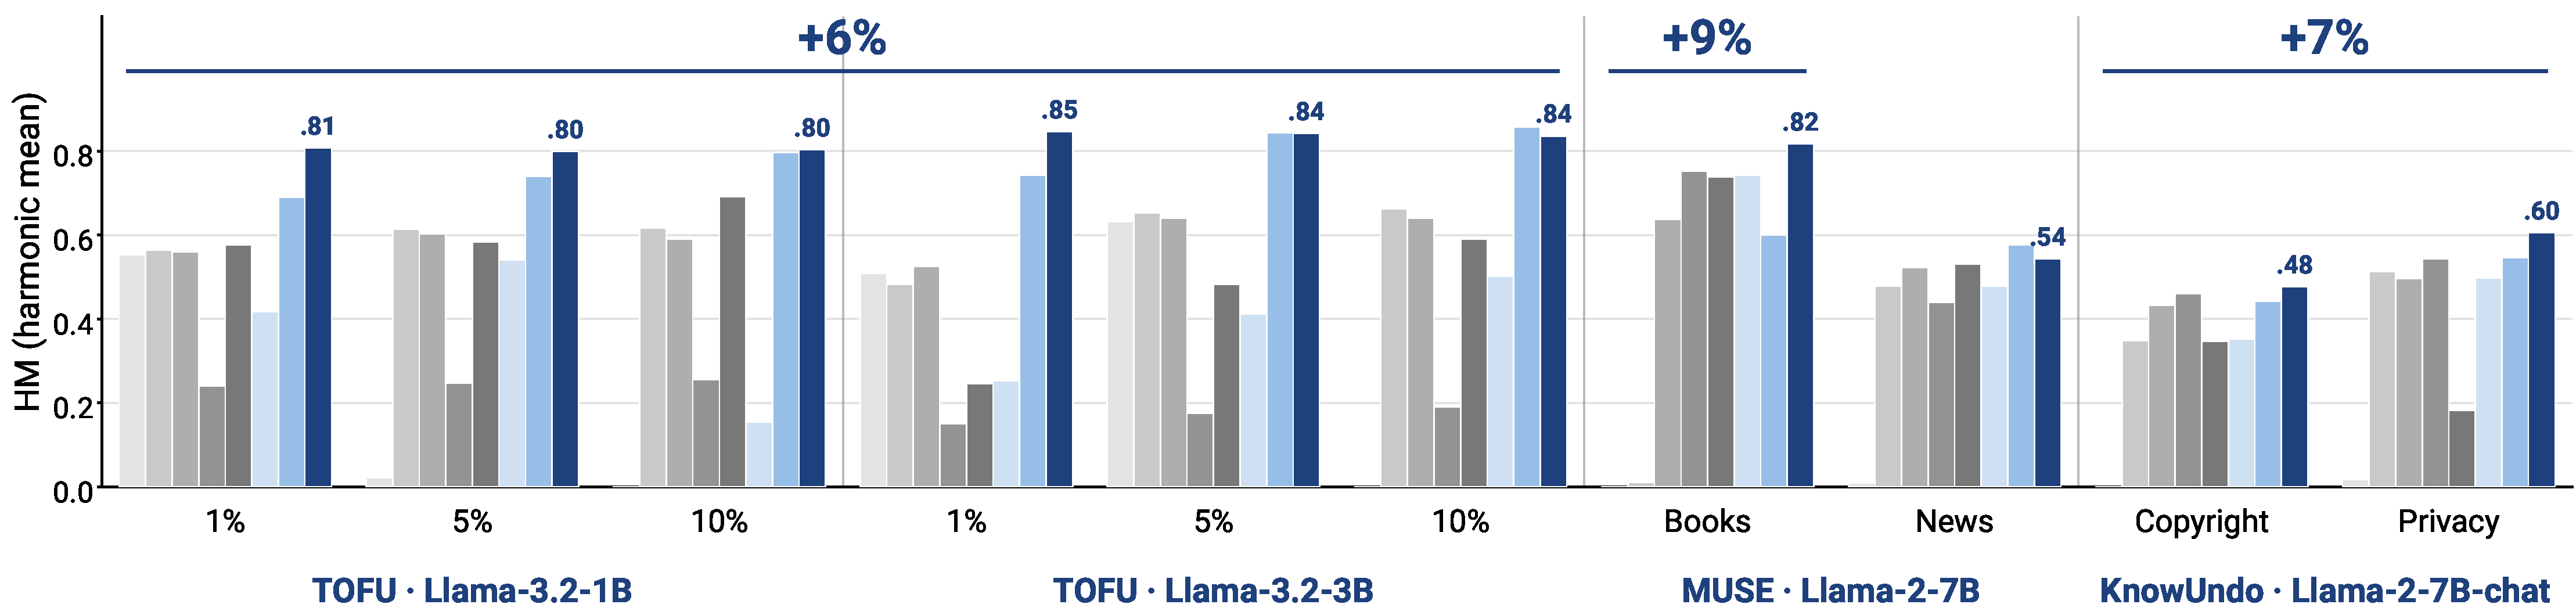
\includegraphics[width=\linewidth]{figures/fig_hm_bars}
        \end{compblock}

        \begin{columns}[T]
          \begin{column}{0.365\linewidth}
            \begin{compblock}[equal height group=e1]{Stable under scaling and repeated requests}
              \centering
              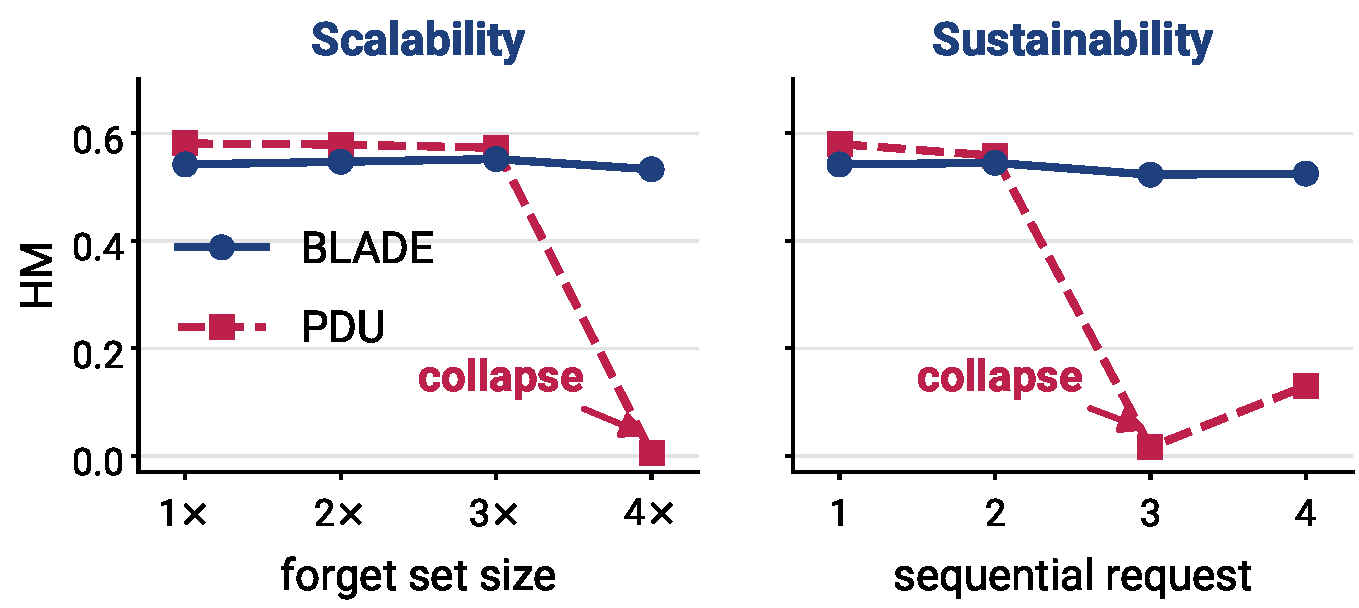
\includegraphics[width=\linewidth]{figures/fig_stress}
            \end{compblock}
          \end{column}
          \begin{column}{0.365\linewidth}
            \begin{compblock}[equal height group=e1]{Training dynamics of \method\ (MUSE Books)}
              \centering
              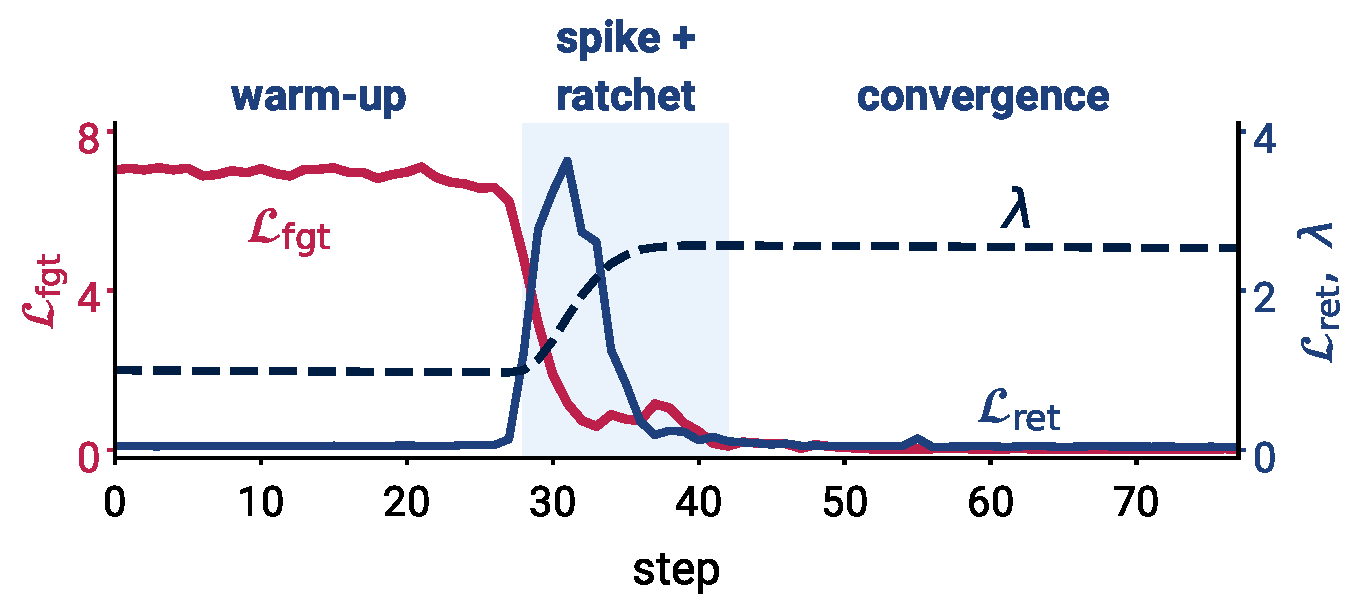
\includegraphics[width=\linewidth]{figures/fig_dynamics}
            \end{compblock}
          \end{column}
          \begin{column}{0.25\linewidth}
            \begin{compblock}[equal height group=e1]{Robust and efficient}
              \raggedright
              \setlength{\tabcolsep}{4pt}\renewcommand{\arraystretch}{1.9}
              \begin{tabular}{@{}c@{\ \ }l@{}}
                {\Large\color{psu-beaver}\faSearch} & \textbf{Extraction:} best HM \\
                {\Large\color{psu-beaver}\faIcon{user-secret}} & \textbf{Jailbreak:} lowest ASR \\
                {\Large\color{psu-beaver}\faIcon{user-shield}} & \textbf{MIA:} no leakage \\
                {\Large\color{psu-beaver}\faTerminal} & \textbf{GCG:} lowest ASR \\
                {\Large\color{psu-beaver}\faMemory} & \textbf{2--5$\times$} less GPU memory \\
              \end{tabular}
            \end{compblock}
          \end{column}
        \end{columns}
      \end{psublock}

      % Row 5 (dynamics + takeaways + QR) parked in parked/row5-dynamics-takeaways.tex

      % ======================= Row 6: references | acknowledgments + QR =======================
      \begin{columns}[T,onlytextwidth]
        \begin{column}{0.60\linewidth}
          \begin{plainblock}[before skip=0pt]{References}
            % Written out by hand (numbers match the superscripts in the benchmark legend).
            \fontsize{21pt}{25pt}\selectfont\raggedright\setlength{\multicolsep}{0pt}
            \newcommand{\refi}[4]{\hangindent=1.3em\hangafter=1\makebox[1.3em][l]{#1.}#2, \textcolor{psu-beaver}{``#3''}, #4.\par\vspace{0.15em}}
            \begin{minipage}[t]{0.49\linewidth}
                \refi{1}{T.~Entesari et al.}{Constrained Entropic Unlearning: A Primal-Dual Framework for Large Language Models}{2025}
                \refi{2}{C.~Fan et al.}{Simplicity Prevails: Rethinking Negative Preference Optimization for LLM Unlearning}{2025}
                \refi{3}{J.~Jang et al.}{Knowledge Unlearning for Mitigating Privacy Risks in Language Models}{2023}
            \end{minipage}\hfill
            \begin{minipage}[t]{0.49\linewidth}
                \refi{4}{H.~Reisizadeh et al.}{BLUR: A Bi-Level Optimization Approach for LLM Unlearning}{2026}
                \refi{5}{R.~Zhang et al.}{Negative Preference Optimization: From Catastrophic Collapse to Effective Unlearning}{2024}
            \end{minipage}
          \end{plainblock}
        \end{column}
        \begin{column}{0.26\linewidth}
          \begin{plainblock}[before skip=0pt]{Acknowledgments}
            \small
            Supported in part by U.S.\ NSF awards \#2438810 and \#2555559, the Amazon Nova AI challenge award,
            and the PSU Frymoyer chairship award. Some results used CloudBank resources, supported by
            U.S.\ NAIRR award \#240336.
          \end{plainblock}
        \end{column}
        \begin{column}{0.12\linewidth}
          \begin{plainblock}[before skip=0pt, halign=center]{Paper}
            \qrcode[height=4.6cm,hyperlink]{https://arxiv.org/abs/2608.22557}\\[0.3ex]
            {\footnotesize\href{https://arxiv.org/abs/2608.22557}{arXiv:2608.22557}}
          \end{plainblock}
        \end{column}
      \end{columns}
    \end{column}

    % right margin
    \begin{column}{0.01\linewidth}
    \end{column}
  \end{columns}
\end{frame}
\end{document}
